\documentclass[conference,12pt]{IEEEtran}
\usepackage{pdflscape}
\usepackage{hyperref}
\usepackage{tabularx}
\usepackage{graphicx, subfigure, amsmath} 
\usepackage{pdfpages}
\usepackage[backend=biber,style=ieee]{biblatex}
\usepackage[section]{placeins}
\addbibresource{References.bib}
\interdisplaylinepenalty=2500

% correct bad hyphenation here
\hyphenation{}


\begin{document}
%
% paper title
\title{Routing IPsec through NAT Gateways using Transport Mode}

\author{
\IEEEauthorblockN{Jeremy Wright}
\IEEEauthorblockA{Arizona State University\\jlwrigh1@asu.edu}
}
\maketitle


\begin{abstract}
\end{abstract}

\begin{IEEEkeywords}
    Transport Mode, Tunnel Mode, IPsec
\end{IEEEkeywords}

\section{Introduction}
IPsec is an end-to-end security protocol for communicating over insecure
channels. IPsec is defined in RFC 4301 \autocite{rfc4301}.  IPsec is a layer
3 protocol according to the OSI Layer Model \autocite{_osi_2014}.  This
  is a key advantage over security protocols at higher levels of abstractions
  such as SSL/TLS.  SSL/TLS requires applications to be specifically designed to
  interact with other SSL/TLS endpoints. IPsec doesn't require the application
  to have any knowledge of security. For some application types, this is an
  enormous advantage, both in terms of application correctness, and in network
  infrastructure roll out. 

\section{IPsec}

IPsec defines two modes of operation transport mode, and tunnel mode. Each mode
has it's own header type. Transport mode uses the Authentication Header (AH), while
Tunnel mode uses the Encapsulated Security Protocol Header. Each header provides varying
levels of service, according to its intended function. Tunnel mode is typically
used for connecting to networks together to form a larger virtual LAN
\autocite{cisco_ipsec}. IPsec meets the 4 tenants of security:
authentication, non-repudiation, integrity, and confidentiality. The integrity
tenant is broken by NAT in the default case. Transport mode is used for connecting 2 end users
together such as in a VPN situation. Transport mode however has additional
issues when using NAT on IPv4 networks \autocite{rfc3022}.

\subsection{Transport Mode}
Transport mode encrypts the entire IP packet, but keeps the routing information
in plain text. The routing information however is incorporated into the hash
value protecting it from tampering. Since the routing information cannot be
changed this causes problems for NAT traversal in IPv4 networks.  On IPv6
networks NAT is not necessary since all addresses are globally routable the
routing information doesn't require change. In the presence of NAT however the
NAT cannot change the source or destination fields, and preserve the integrity
of the packet. Tunnel mode provides a method for dealing with this.

\begin{figure}
\centering
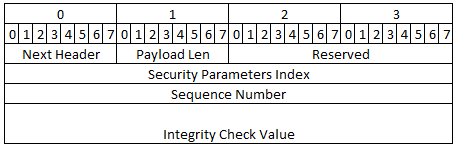
\includegraphics[width=0.4\textwidth]{AH.png}
\caption{IPsec: Authentication Header}
\label{fig:ah}
\end{figure}

\subsection{Tunnel Mode}
Tunnel Mode uses the ESP header (Figure~\ref{fig:esp}) to wrap the desired IP
packet. The encapsulated IP package is encrypted, and the outer header defines
mutable, and immutable fields available for NAT \autocite{rfc4301}.  In tunnel
mode,  additional overhead since it doesn't use an additional IP
Packet to wrap the security packet as IPsec Tunnel Mode requires. 

\begin{figure}
\centering
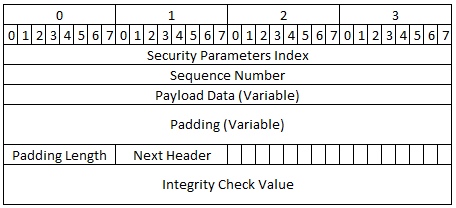
\includegraphics[width=0.4\textwidth]{ESP.png}
\caption{IPsec: Encapsulated Security Payload Header}
\label{fig:esp}
\end{figure}

\section{NAT-T Traversal}
RFC3947 provides a mechanism to use IPsec in the presence of a NAT gateway
\autocite{rfc3947}.  

\section{Alternative with Generic Routing Protocol}
Another option is to use the Generic Routing Protocol to route IPsec packets
through the NAT \autocite{rfc2784}. This may be especially useful if the NAT in question isn't
compliant and breaks the IPsec integrity packets.  Also for applications where
the user must act as both a server and a client, such as video games where
multi-player hosts connect to one another, or in peer-to-peer. in this case, the
NAT will likely drop in coming connections, or the NAT may be handing
a connection on port 500 at that instant, and the incoming connection would be
ambiguous \autocite{rfc3715}
. In this case connecting to the correct internal host would be
unlikely. 

Generic Routing Protocol (GRP), is a layer 3 protocol which encapsulates any
other protocol.  Since this protocol is unsecured, the NAT is free to mutate
fields and operate as normal.  However the receiver can accept the GRP packets
peel off the encapsulated inner packets, and continue routing within the
network \autocite{rfc3193}
. 

\section{Conclusion}
Traditionally, when configuring IPsec, one would use Tunnel Mode to connect to
large networks together creating a larger virtual LAN. For remote users
connecting to a publicly accessible server, transport mode maybe more useful.
However to create a secure connection between two end users in a peer-to-peer
fashion, one can look at defining
a new protocol based on the GRP, to route their custom secure clients through
Network Address Translators.


\printbibliography
\end{document}


